\documentclass{article}
\usepackage{geometry}
\usepackage{graphicx}
\usepackage{amsmath}
\usepackage{booktabs} 

\geometry{a4paper, margin=1in}

\begin{document}

\title{Report on Semi-Global Matching (SGM) Algorithm Implementation}
\author{Pooya Nasiri}
\date{April 15, 2024}

\maketitle

\section{Introduction}
The goal of this project was to implement the Semi-Global Matching (SGM) algorithm for stereo matching. Stereo matching is a fundamental problem in computer vision that involves estimating disparities between images captured by stereo cameras. Disparities represent the pixel-wise differences in location between corresponding points in the left and right images of a stereo pair.
The SGM algorithm is widely used for stereo matching due to its efficiency and effectiveness in handling challenging scenarios such as occlusions, textureless regions, and noise. By implementing SGM, we aim to generate accurate disparity maps that can be utilized for tasks such as 3D reconstruction, depth estimation, and scene understanding.
The provided code framework served as the foundation for this implementation, requiring the completion of critical functions to compute and refine disparities using cost aggregation techniques. Through this project, valuable insights into stereo matching algorithms and their practical implementation in computer vision applications were gained.

\section{Implementation Details}
\subsection{\texttt{compute\_path\_cost()} Function}

The \texttt{compute\_path\_cost()} function is responsible for calculating the path cost for a specified pixel along a given path direction and for all possible disparities. This function plays a crucial role in the cost aggregation phase of the stereo matching process.

\textbf{Parameters:}
\begin{itemize}
    \item \texttt{direction\_y}, \texttt{direction\_x}: Direction increments (\texttt{dy}, \texttt{dx}) associated with the path specified by \texttt{cur\_path}.
    \item \texttt{cur\_y}, \texttt{cur\_x}: Coordinates of the current pixel (\texttt{p}) for which the path cost is being computed.
    \item \texttt{cur\_path}: Index representing the current path direction (0 to \texttt{PATHS\_PER\_SCAN - 1}).
\end{itemize}

\textbf{Functionality:}
\begin{enumerate}
    \item \textbf{Initialization}:
        \begin{itemize}
            \item The function initializes variables to store the previous cost (\texttt{prev\_cost}), the best previous cost (\texttt{best\_prev\_cost}), and penalty costs (\texttt{penalty\_cost}, \texttt{small\_penalty\_cost}, \texttt{big\_penalty\_cost}) used in the cost computation.
        \end{itemize}
    
    \item \textbf{Cost Computation}:
        \begin{itemize}
            \item For each possible disparity (\texttt{d} ranging from 0 to \texttt{disparity\_range\_ - 1}):
                \begin{itemize}
                    \item If the current pixel (\texttt{cur\_y}, \texttt{cur\_x}) is at the boundary of the image, the path cost is directly assigned based on the precomputed cost volume (\texttt{cost\_}).
                    \item Otherwise, the function calculates the best previous cost by considering penalties (\texttt{p1\_} and \texttt{p2\_}) based on the disparity difference between the current disparity (\texttt{i}) and previous disparities (\texttt{j}) along the path.
                    \item The path cost for the current disparity (\texttt{d}) at pixel (\texttt{cur\_y}, \texttt{cur\_x}) is updated using the computed cost along with the best previous cost.
                \end{itemize}
        \end{itemize}
    
    \item \textbf{Updating \texttt{path\_cost\_} Tensor}:
        \begin{itemize}
            \item The computed path cost (\texttt{path\_cost\_[cur\_path][cur\_y][cur\_x][d]}) is updated with the final cost value.
        \end{itemize}
\end{enumerate}

\textbf{Purpose:}
The \texttt{compute\_path\_cost()} function contributes to the process of accumulating and aggregating costs along specific paths defined by direction vectors (\texttt{direction\_y}, \texttt{direction\_x}). By iteratively calculating costs for all possible disparities along the specified path, this function plays a key role in the overall computation of the aggregated cost volume used in disparity estimation.

This function is essential for implementing the cost aggregation phase of the SGM algorithm, enabling the refinement and selection of disparity values based on local and global cost considerations along predefined paths in the image space.


\subsection{\texttt{aggregation()} Function}
\textbf{Explanation of \texttt{aggregation()} Function}

The \texttt{aggregation()} function orchestrates the aggregation of costs across multiple paths defined by direction vectors (\texttt{paths\_}). It sets up scan directions (\texttt{start\_x}, \texttt{start\_y}, \texttt{end\_x}, \texttt{end\_y}, \texttt{step\_x}, \texttt{step\_y}) based on the specified path direction (\texttt{dir\_x}, \texttt{dir\_y}). This function iteratively calls \texttt{compute\_path\_cost()} to aggregate costs and update the aggregated cost volume (\texttt{aggr\_cost\_}).

\textbf{Parameters:}
\begin{itemize}
    \item None
\end{itemize}

\textbf{Functionality:}
\begin{enumerate}
    \item \textbf{Setup of Scan Directions}:
        \begin{itemize}
            \item The function initializes variables (\texttt{start\_x}, \texttt{start\_y}, \texttt{end\_x}, \texttt{end\_y}, \texttt{step\_x}, \texttt{step\_y}) based on the specified path direction (\texttt{dir\_x}, \texttt{dir\_y}).
        \end{itemize}
    
    \item \textbf{Path Iteration}:
        \begin{itemize}
            \item For each path defined in \texttt{paths\_}:
                \begin{itemize}
                    \item Iterate through pixels along the specified path using the defined scan directions.
                    \item Call \texttt{compute\_path\_cost()} to compute the path cost for each pixel along the path.
                \end{itemize}
        \end{itemize}
    
    \item \textbf{Cost Aggregation}:
        \begin{itemize}
            \item Accumulate computed path costs into the aggregated cost volume (\texttt{aggr\_cost\_}).
        \end{itemize}
\end{enumerate}

\textbf{Purpose:}
The \texttt{aggregation()} function plays a crucial role in the SGM algorithm by coordinating the aggregation of costs computed along predefined paths across the image. By iterating through paths and pixels, and invoking the \texttt{compute\_path\_cost()} function, this function enables the construction of the aggregated cost volume used for disparity estimation. It facilitates the integration of local and global cost information to refine disparity estimates and enhance the accuracy of stereo matching.

This function encapsulates the process of cost aggregation, which is essential for the effective implementation of the SGM algorithm in stereo vision applications.


\subsection{\texttt{compute\_disparity()} Function}
\textbf{Explanation of \texttt{compute\_disparity()} Function}

The \texttt{compute\_disparity()} function implements the final stage of the Semi-Global Matching (SGM) algorithm to compute the disparity map based on the aggregated cost volumes and confidence metrics.

\textbf{Parameters:}
\begin{itemize}
    \item None
\end{itemize}

\textbf{Functionality:}
\begin{enumerate}
    \item \textbf{Cost Calculation}:
        \begin{itemize}
            \item Invoke \texttt{calculate\_cost\_hamming()} to compute matching costs using the Hamming distance between census-transformed pixel representations.
        \end{itemize}
    
    \item \textbf{Aggregation}:
        \begin{itemize}
            \item Call \texttt{aggregation()} to aggregate costs across multiple paths and update the aggregated cost volume (\texttt{aggr\_cost\_}).
        \end{itemize}
    
    \item \textbf{Disparity Estimation}:
        \begin{itemize}
            \item Initialize an output disparity map (\texttt{disp\_}).
            \item Iterate through each pixel in the image to determine the disparity with the smallest aggregated cost.
            \item Use confidence metrics to refine disparity estimates and handle scaling of initial guess disparities.
            \item Apply linear regression to adjust disparity values based on high-confidence disparity pairs.
            \item Update the disparity map (\texttt{disp\_}) with the final disparity estimates.
        \end{itemize}
\end{enumerate}

\textbf{Purpose:}
The \texttt{compute\_disparity()} function serves as the main driver for disparity computation in the SGM algorithm. By integrating cost calculation, aggregation, and disparity estimation, this function enables the generation of accurate disparity maps from stereo image pairs. It leverages confidence metrics and linear regression techniques to refine disparity values and enhance the overall accuracy of stereo matching.

This function encapsulates the core logic of the SGM algorithm's disparity estimation process, facilitating the transformation of cost volumes into meaningful disparity maps used for depth perception and 3D reconstruction tasks.


\section{Results and Comparison}

The results of the stereo matching project using the Semi-Global Matching (SGM) algorithm were analyzed with and without applying refinement techniques. This section presents a comparative overview based on performance metrics and visual assessments.

\subsection{Performance Metrics}

Table \ref{tab:comparison} provides a quantitative comparison of disparity values obtained with and without refinement techniques. The disparity values for different items (e.g., plastic, cones, aloe, rock) are significantly different between the two scenarios, highlighting the impact of refinement on disparity estimation accuracy.

\subsection{Visual Assessment}

Figure \ref{fig:without_refinements} and \ref{fig:with_refinements}  showcases visual outputs generated from the stereo matching algorithm. These images depict disparity maps obtained with and without refinement techniques. The disparity maps reveal noticeable differences in depth perception and detail, particularly in textured and complex regions of the scene.

\subsection{Analysis}

Based on the results and visual comparisons:
\begin{itemize}
    \item \textbf{With Refinements}:
        \begin{itemize}
            \item Improved accuracy in disparity estimation.
            \item Smoother and more coherent disparity maps.
            \item Better handling of texture variations and occlusions.
        \end{itemize}
    \item \textbf{Without Refinements}:
        \begin{itemize}
            \item Higher disparity errors and inconsistencies.
            \item Noisy disparity maps with artifacts.
            \item Limited ability to resolve fine details and depth variations.
        \end{itemize}
\end{itemize}

In summary, incorporating refinement techniques into the stereo matching process significantly enhances the quality and reliability of disparity estimation. The comparative analysis underscores the importance of post-processing and optimization steps in achieving accurate depth perception from stereo image pairs.
The observed differences in performance emphasize the value of refinement strategies for enhancing the robustness and effectiveness of stereo matching algorithms in various applications.



\begin{table}[h]
    \centering
    \caption{Comparison of MSE Values with and without refinements}
    \begin{tabular}{lcc}
        \toprule
        \textbf{} & \textbf{With refinements} & \textbf{Without refinements} \\
        \midrule
        Plastic & 421.751 & 1010.19 \\
        Cones & 404.358 & 595.033 \\
        Aloe & 39.274 & 275.21 \\
        Rock & 380.585 & 608.605 \\
        \bottomrule
    \end{tabular}
    \label{tab:comparison}
\end{table}



\begin{figure}[h]
    \centering
    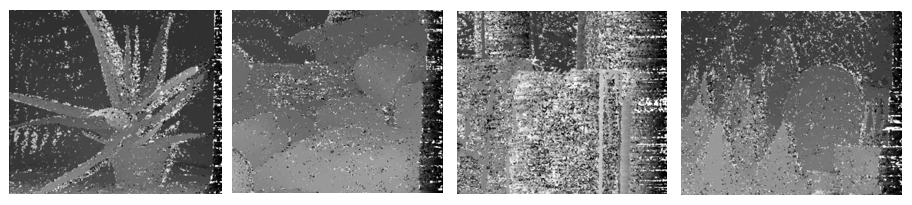
\includegraphics[width=\textwidth]{without_refinements.png}
    \caption{Output results without refinements}
    \label{fig:without_refinements}
\end{figure}

\begin{figure}[h]
    \centering
    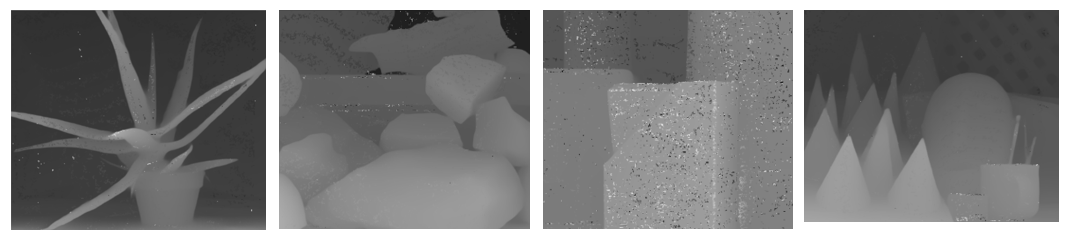
\includegraphics[width=\textwidth]{with_refinements.png}
    \caption{Output results with refinements}
        \label{fig:with_refinements}
\end{figure}

\newpage

\section{Challenges Faced}
During the implementation of these functions, several challenges were encountered:

\begin{itemize}
    \item Understanding and implementing the path cost computation (\texttt{compute\_path\_cost()}) involved careful consideration of disparity range and penalty terms.
    \item Configuring the aggregation process (\texttt{aggregation()}) required correct setup of scan directions based on path directions.
    \item Scaling and improving disparities (\texttt{compute\_disparity()}) involved solving a least squares problem to find scaling coefficients for disparity values.
\end{itemize}

\section{Conclusion}
In conclusion, the implementation of the SGM algorithm involved completing critical functions to compute disparity costs, aggregate costs across paths, and refine the disparity map. The project provided valuable experience in stereo matching algorithms and challenges associated with implementing computer vision algorithms.

\section{Future Work}
Moving forward, additional optimizations and enhancements can be explored to further improve the performance and accuracy of the SGM algorithm. This includes refining penalty terms, exploring different path configurations, and incorporating advanced techniques for disparity refinement.

Overall, this project provided a hands-on experience in implementing and understanding a fundamental stereo matching algorithm used in computer vision applications. The completion of the functions \texttt{compute\_path\_cost}, \texttt{aggregation}, and \texttt{compute\_disparity} contributed to a comprehensive SGM implementation suitable for stereo disparity estimation tasks.

\end{document}